\documentclass[fleqn, 12pt]{article}

\usepackage[utf8]{inputenc}
\usepackage[bulgarian]{babel}
\usepackage{amsmath}
\usepackage{amssymb}
\usepackage{booktabs}
\usepackage{fancyhdr}
\usepackage{amsthm}
\usepackage{graphicx}

\theoremstyle{definition}
\newtheorem{theorem}{Tеорема}[subsection]
\newtheorem{example}{Пример}[subsection]
\newtheorem{definition}{Дефиниция}[subsection]

\title{Физика}
\author{Exonaut}

\pagestyle{fancy}
\fancyhf{}
\lhead{\rightmark}
\rhead{\thepage}
\cfoot{}
\renewcommand{\headrulewidth}{0pt}

\begin{document}
\maketitle
\pagenumbering{gobble}
\newpage
\pagenumbering{arabic}

\tableofcontents
\newpage

\section{Лекция 1: Кинематика}
Механиката се дели на: 
\begin{itemize}
	\item Кинематика: описва движението, без да се интересува от причините, които го пораждат.
	\item Динамика: изучава законите за движение и причините, които го предизвикват.
	\item Статика: изучава условията за равновесие на телата.
\end{itemize}

\subsection{Основни понятия}

\begin{itemize}
	\item Материална точка: тяло, чиито форма и размери могат да се пренебрегнат при изучаване на движението му.
	\item Отправно тяло: тяло, спрямо което отчитаме движението.
	\item Отправна система: състои се от отправно тяло, координатна система и часовник.
	\item Радиус вектор: вектор от началото на отправната система до материалната точка. Означава се с $\vec{r}(t)$
	\item Траектория: линията, описвана от материалната точка при движението й.
	\item Път: дължината на траекторията от началното до крайното положение.
	\item Преместване: вектор от началното до крайното положение.
\end{itemize}

\subsection{Праволинейно движение}
Като начало ще разгледаме движението само по едно направление, например по оста x. Такова движение се нарича праволинейно.

\subsubsection{Средна скорост}
Средна скорост: преместването по $\Delta x$ разделена на интервала време $\Delta t$, или $V(t) = \dfrac{\Delta x}{\Delta t}$.

\subsubsection{Моментна скорост}
Ако интеравала е много малък $(\Delta t \rightarrow 0)$ скоростта се нарича моментна : $V(t) = \lim\limits_{\Delta t \rightarrow 0}\dfrac{\Delta x}{\Delta t} = \dfrac{dx}{dt}$. $dx$ е много малко преместване извършено в за много малък интервал от време $dt$.\\
\\
\textbf{Моментната скорост е първа производна на радиус-вектора по времето.} или 
$$V(t) = \dfrac{d \vec{r}}{dt}$$
$$V = \left[ \dfrac{m}{s}\right] = \left[ \dfrac{km}{h}\right], \quad 1\dfrac{m}{s} = 3,6 \dfrac{km}{h} $$

\subsubsection{Средно ускорение}
Средно ускорение наричаме изменението на скоростта $\Delta V$ , разделено на интервала време, за който е извършено това изменение: $a(t) =\dfrac{\Delta V}{\Delta t}$.

\subsubsection{Моментно ускорение}
Ако интеравала е много малък $(\Delta t \rightarrow 0)$ ускорението се нарича моментно : $a(t) = \lim\limits_{\Delta t \rightarrow 0}\dfrac{\Delta V}{\Delta t} = \dfrac{dV}{dt}$.\\
\\
\textbf{Моментното ускорение е първа производна на скоростта по времето и втора производна на радиус-вектора по времето: } или 
$$a(t) =  \dfrac{dV}{dt} = \dfrac{d^2 \vec{r}}{dt^2}$$
$$a = \left[ \dfrac{m}{s^2} \right]$$

\begin{example}
Тяло се движи по закон $x = 5t^3 + 2t^2 + 1$. Да се намери скоростта и ускорението в момента $t = 1s$. \\
Решение: \\
\begin{gather*}
V(t) = \dfrac{dx}{dt}, \quad a(t) = \dfrac{dV}{dt} \\
V(t) = 5 \cdot 3 \cdot t^{3-1} + 2 \cdot 2 \cdot t^{2-1} + 0 = 15 \cdot t^2 + 4\cdot t \\
a(t) = 15\cdot 2 \cdot t^{2-1} + 4 = 30 \cdot t + 4 \\
V(1) = 15 \cdot 1^2 + 4 \cdot 1 = 15 + 4 = 19 \dfrac{m}{s} \\
a(1) = 30 \cdot 1 + 4 = 30 + 4 = 34 \dfrac{m}{s^2}
\end{gather*}
\end{example}

\subsection{Движение с постоянна скорост}
Нека материална точка се движи с начална скорост $V_0$ . В момента $t_0 = 0$ тя започва да се движи с постоянно ускорение $a = const$. В някакъв по-късен момент $t$ материалната точка се движи със скорост $V$. От дефиницията за ускорение  $ a =\dfrac{\Delta V}{\Delta t}$ можем да запишем 
$$a = \dfrac{V - V_0}{t - t_0} = \dfrac{V - V_0}{t}$$
$$a = \dfrac{V - V_0}{t} \implies V - V_0 = at \implies V = V_0 + at$$
Изразът за зависимостта на скоростта от времето($V = V_0 + at$) се нарича закон за скоростта. \\
\\
Нека материална точка започва да се движи в момента $t_0 - 0$ от положение с координата $x_0$ с постоянна скорост  $V_0 = const$. В някакъв по-късен момент $t$ материалната точка има координата $x$. От дефиницията за скорост  $V_0 = \dfrac{\Delta x}{\Delta t}$ можем да запишем $V_0 = \dfrac{x-x_0}{t - t_0}$ или $x = x_0 + V_0(t-t_0)$, но $t_0 = 0$ от където следва 
$$x = x_0 + V_0t$$
При движение с постоянно ускорение $a$ към горния израз се добавя още един член, отчитащ промяната в скоростта: 
$$x = x_0 + V_0t + \dfrac{at^2}{2}$$
Изразът, даващ зависимостта на радиус-вектора от времето се нарича закон за движение. \\
Знаците пред скоростта и ускорението в горните изрази могат да бъдат като положителни, така и отрицателни. Знакът е положителен, ако посоката на $V$ или а съвпада с посоката на оста х и отрицателен, ако посоката е противоположна на оста х.\\
Ако ускорението е константа и скоростта на тялото нараства с времето, движението се нарича \textit{равноускорително}. Ако скоростта на тялото намалява – \textit{равнозакъснително}, а ако ускорението е нула и скоростта на тялото не се променя, говорим за \textit{равномерно} движение.

\begin{example}
Кола се движи със скорост $V_0$ . След задействане на спирачката, колата започва да се движи равнозакъснително с ускорение $a$ и скоростта на колата намалява до $V$. Намерете спирачния път.\\
Решение:
$$V = V_0 - at$$
$$x = V_0t - \dfrac{at^2}{2}$$
Oт първото равенство имаме $t = \dfrac{V_0 - V}{a}$ и заместваме във второто равенство
\begin{gather*}
x = V_0 \dfrac{V_0 - V}{a} - \dfrac{1}{2}a \left( \dfrac{V_0 - V}{a}\right)^2 \\
x = \dfrac{V_0 ^2 - VV_0}{a} -  \dfrac{a}{2}  \left( \dfrac{V_0 ^2 - 2VV_0 + V^2}{a^2}\right)\\ 
x =\dfrac{V_0 ^2 - VV_0}{a} - \dfrac{a(V_0 ^2 - 2VV_0 + V^2)}{2a^2}\\
x = \dfrac{2(V_0 ^2 - VV_0)}{2a} - \dfrac{V_0 ^2 - 2VV_0 + V^2}{2a}\\
x = \dfrac{2V_0 ^2 - 2VV_0 - V_0 ^2 + 2VV_0 - V^2}{2a}\\
x = \dfrac{V_0 ^2 - V^2}{2a}
\end{gather*}
\end{example}

\begin{example}
Тяло е хвърлено вертикално нагоре от височина $h_0 = 1m$ с начална скорост $V_0 = 10 \dfrac{m}{s}$. След колко време тялото ще достигне максимална височина? До каква максимална височина ще се издигне тялото? След колко време и с каква скорост тялото ще падне до $h = 0$. \\
Решение: \\
$g = 9,8 \dfrac{m}{s^2} \approx 10 \dfrac{m}{s^2}$. \\
$$V = V_0 - gt$$
$$y = h_0 + V_0t - \dfrac{gt^2}{2}$$
Знакът пред $V_0$ е положителен, защото посоката й съвпада с посоката на оста $y$, а знакът пред $g$ е отрицателен, защото посоката му е противоположна на оста $y$.Когато тялото се издига, скоростта му намалява, в най-високата точка става нула, след което тялото започва да пада, скоростта му става отрицателна, понеже е насочена срещу оста $y$. В най-високата точка $V = 0$  или $0 = V_0 - gt$. От тук намираме времето, за което тялото ще достигне най-високата точка $t = \dfrac{V_0}{g} = \dfrac{10}{10} = 1s$. Заместваме това време в израза за y за да получим максималната височина:

\begin{gather*}
h_{max} = h_0 + V_0t -  \dfrac{gt^2}{2} = 1+ 10 \cdot 1 -  \dfrac{10 \cdot 1^2}{2} = 11 - 5 = 6m\\
h = 0  \implies y = 0\\
0 = h_0 + V_0t - \dfrac{gt^2}{2} \\
0 = 1 + 10t -  \dfrac{10t^2}{2}\\
-5t^2 + 10t  + 1 = 0 \\
D = 10^2 - 4 \cdot (-5) \cdot 1 = 100 + 20 = 120 \\
t_{1,2} = \dfrac{-10 \pm \sqrt{120}}{2 \cdot (-5)} = \dfrac{-10 \pm 2\sqrt{30}}{-10} = \dfrac{-5 \pm \sqrt{30}}{-5}\\
t_1 = \dfrac{-5 -\sqrt{30}}{-5} \approx -0.1 s\\
t_2 = \dfrac{-5 +\sqrt{30}}{-5} \approx 2.1 s
\end{gather*}
Физичен смисъл има само положителното време. Заместваме го в израза за скоростта $V = V_0 - gt = 10 - 10 \cdot 2.1 = -11 m/s$ Това е скоростта, с която тялото пада на земята. Тя е отрицателна, защото е насочена срещу оста $y$.
\end{example}

\subsection{Движение при произволна форма на траекторията}
Когато движението не е праволинейно, скоростта и ускорението се записват за всяка от компонентите на радиус-вектора: 
$$V_x = \dfrac{dx}{dt}, \quad V_y = \dfrac{dy}{dt}, \quad V_z = \dfrac{dz}{dt} \qquad \vec{V} = \dfrac{d\vec{r}}{dt}$$
Скоростта $\vec{V}$ е векторна величина - тя се характеризира с големина и посока. Големината на скоростта се определя от координатите на скоростта (по Питагоровата теорема) $V = \sqrt{V_x^2 + V_y^2 + V_z^2}$ \\
Аналогично: 
$$\vec{a} = \dfrac{d\vec{V}}{dt} = \dfrac{d^2 \vec{r}}{dt^2}$$ 
Тъй като скоростта е вектор, тя може да се изменя поради промяна на големината и поради промяна на посоката си.\\
Ускорението, дължащо се на изменение на скоростта по големина се нарича тангенциално ускорение $\vec{a_\tau}$. То има посока, съвпадаща с направлението на скоростта.\\
Ускорението, дължащо се на изменение на скоростта по посока се нарича нормално ускорение $\vec{a_n}$. То има посока, перпендикулярна на направлението на скоростта. Може да се покаже, че $\vec{a_n} = \dfrac{V^2}{R}$, като R е радиусът на кривината на траекторията в разглежданата точка. \\
От казаното по-горе е ясно, че при праволинейно движение нормалното ускорение е винаги нула. При движение по крива, дори и с постоянна скорост, нормалното ускорение е различно от нула.
Пълното ускорение се получава като векторна сума от тангенциалното и нормалното ускорение:
$$\vec{a} =\vec{a_\tau} + \vec{a_n}$$
При постоянно ускорение законът за скоростта и за движение се записват във векторен вид: 
$$\vec{V} = \vec{V_0} + \vec{a}t$$
$$\vec{r} = \vec{r_0} + \vec{V_0}t + \dfrac{\vec{a}t^2}{2}$$
След това се записват уравненията за всяка от компонентите на векторите.

\begin{example}
Тяло е хвърлено под ъгъл $\alpha = 30^\circ $ спрямо хоризонта с начална скорост 
$V_0 = 10 \dfrac{m}{s}$. Намерете максималната височина, до която се издига тялото и разстоянието, което то прелита. \\
Решение: $\vec{r_0} = 0$. \\
$$\vec{V} = \vec{V_0} + \vec{g}t$$
$$\vec{r} = \vec{V_0}t + \dfrac{\vec{g}t^2}{2}$$
Всеки от векторите може да бъде разложен на две компоненти $x$и $y$. \\
По оста $x$: $V_x = V_{0x}, \quad x = V_{0x}t$ \\
По оста $y$: $V_y = V_{0y} - gt, \quad y = V_{0y}t - \dfrac{\vec{g}t^2}{2}$ \\
Тук сме взели предвид, че по оста $x$ няма ускорение, а по оста $y$ ускорението е $g$, насочено надолу, в посока обратна на оста $y$(и затова с отрицателен знак). \\
$$V_{0x} = V_0 \cos{30^\circ} = \dfrac{\sqrt{3}}{2}V_0 \quad V_{0y} = V_0 \sin{30^\circ} = \dfrac{V_0}{2}$$
В най високата точка $V_y$ е равна на 0: $0 = V_{0y} - gt$ и времето за което тялото достига максимална височина е $t = \dfrac{V_{0y}}{g}$
Заместваме това време в израза за y и получаваме 
\begin{gather*}
y_{max} = V_{0y} \dfrac{V_{0y}}{g} - \dfrac{g}{2} \cdot \left(  \dfrac{V_{0y}}{g} \right)^2 \\
y_{max} = \dfrac{V_{0y}^2}{g} - \dfrac{1}{2} \cdot \dfrac{V_{0y}^2}{g}\\
y_{max} = \dfrac{1}{2} \cdot \dfrac{V_{0y}^2}{g} =  \dfrac{1}{2} \cdot \dfrac{\left( \dfrac{10}{2} \right)^2}{10} = \dfrac{5^2}{20} = \dfrac{25}{20} = 1.25m
\end{gather*}
\end{example}
В общия случай, когато ускорението не е постоянно, законът за скоростта се получава с интегриране. 
$$\vec{a} =  \dfrac{d\vec{V}}{dt} \Leftrightarrow d\vec{V} = \vec{a}dt$$
$$\vec{V} = \int _0 ^ t  \vec{a}(t)dt + \vec{V_0}$$
Аналогично закона за движение : 
$$\vec{V} =  \dfrac{d\vec{r}}{dt} \Leftrightarrow d\vec{r} = \vec{V}dt$$
$$\vec{r} = \int _0 ^ t  \vec{V}(t)dt + \vec{r_0}$$
Ще използваме този резултат за да получим закона за движение при постоянно ускорение. При движение с постоянно ускорение  
$$\vec{V} = \int _0 ^ t  \vec{a}dt + \vec{V_0} = \vec{V_0} + \vec{a} \int _0 ^ t dt = \vec{V_0} + \vec{a}t$$
Заместваме този резултат в $\vec{r} = \int _0 ^ t  \vec{V}(t)dt + \vec{r_0}$ и получаваме 
$$\vec{r} = \int _0 ^ t (\vec{V_0} + \vec{a}t) dt + \vec{r_0} = \vec{r_0} + \int _0 ^ t \vec{V_0} dt + \int _0 ^ t \vec{a}t dt$$
$$ \vec{r} = \vec{r_0} + \vec{V_0}t +\dfrac{\vec{a}t^2}{2} $$

\newpage

\section{Лекция 2: Динамика на материална точка}

\subsection{Принципи на механиката (Принципи на Нютон)}
 
\subsubsection{Първи принцип}

\textbf{Всяко тяло запазва състоянието си на покой или на праволинейно равномерно движение, докато външно въздействие не го изведе от това състояние.}\\
Този принцип не е в сила за всички отправни системи. Отправните системи, за които той е в сила, се наричат \textit{инерциални отправни системи}. \\
Величината, която количествено характеризира взаимодействието между телата, се нарича сила. Силата е векторна величина – има големина, посока и приложна точка. Означава се с буквата F. Мерната единица за сила е нютон N.\\
Телата притежаватсвойството инертност – съпротивляват се на въздействие, което се стреми да ги извади от състоянието им на покой или на праволинейно равномерно движение. Това свойство се характеризира с величината маса m. Измерва се в килограми kg. Колкото по-голяма масата на едно тяло, толкова по-трудно е да изменим неговата скорост. \\
Произведението на масата и скоростта на едно тяло се нарича импулс $$\vec{p} = m \vec{V}$$
Mерната единица за импулс е  $ \dfrac{kg \cdot m}{s} $

\subsubsection{Втори принцип}
\textbf{Първата производна на импулса по времето е равна на силата, действаща на тялото.}
$$\vec{F} = \dfrac{d \vec{p}}{dt}$$
Ако масата не се променя можем да запишем
$$\vec{F} = \dfrac{d \vec{p}}{dt} = \dfrac{d m\vec{V}}{dt} = m \dfrac{d\vec{V}}{dt} = m \vec{a}$$
Mерната единица за сила $N = \dfrac{kg \cdot m}{s^2}$, Когато на тялото
действат няколко сили, $\vec{F}$ е векторната сума на тези сили.

\subsubsection{Трети принцип}
\textbf{Силите на взаимодействие между две тела са равни по големина и противоположни по посока.}

\subsection{Някои видове сили}

\subsubsection{Гравитационна сила}
Законът на Нютон за гравитацията гласи: \textit{Между всеки две материални точки действа сила на привличане, която е правопропорционална на произведението на масите им и обратно пропорционална на квадрата на разстоянието между тях.} \\
$$F = \gamma \dfrac{m_1 m_2}{r^2}$$
$\gamma = 6.67 \cdot 10^{-11} \dfrac{N \cdot m^2}{kg^2}$, $m_1, m_2$ - масите на двете материални точки, а r - разстоянието между тях. 

\begin{example}
Две тела с маси $m_1 =m_2 = 100 kg$ са разположени на разстояние r = 1 m.Намерете силата на привличане. \\
Решение: \\
$$F = \gamma \dfrac{m_1 m_2}{r^2} =  6.67 \cdot 10^{-11}  \dfrac{100 \cdot 100}{1^2} = 6.67 \cdot 10^{-7} N$$
\end{example}


\subsubsection{Сила на тежестта}
Разглеждаме тяло в близост до земната повърхност. Гравитационната сила, действаща на тялото в този случай ще означим с G, масата Земята с M, а разстоянието до центъра на Земята с R. Записваме закона за гравитацията:
$$G = \gamma \dfrac{mM}{R^2} = m \left( \gamma \dfrac{M}{R^2} \right)$$
$\gamma \dfrac{M}{R^2} $ е еднаква за всички тела величина, която се означава с g и се нарича земно ускорение. Стойността на $g \approx 9.8 \dfrac{m}{s^2}$ е измерена експериментално. Оттук може да запишем за силата на тежестта:
$$G = mg$$
При принципите на Нютон въведохме масата като мярка за инерчните свойства на телата. Тук даваме още едно определение за масата – тя характеризира гравитационните свойства на телата. Масата в  $\vec{F} = m \vec{a}$ се нарича инертна маса, а масата в $G = mg$ - тежка маса. Съгласно съвременната физика тежката и инертната маса са еквивалентни.

\subsubsection{Реакция на опората}
Разглеждаме книга поставена на един чин. Книгата действа на чина със силата на тежестта $G = mg$ , насочена надолу. Съгласно третия принцип на Нютон и чинът действа на книгата със същата по големина сила, но насочена нагоре. Тази сила се нарича реакция на опората и ще я означаваме с N. В крайна сметка на книгата действат две равни по големина сили G и N , насочени в противоположни посоки. Тяхната векторна сума е нула и затова книгата остава в покой. \\
Реакцията на опората винаги е перпендикулярна на повърхността, на която е поставено тялото.
 
\begin{example}
Тяло се спуска без триене по равнина, наклонена под ъгъл $\theta$. Определете ускорението на тялото и реакцията на опората. \\
Решение: \\
Избираме отправна система, при която оста х е успоредна на равнината, а оста у е перпендикулярна на равнината. Записваме втория принцип на Нютон $\vec{F} = m \vec{a}$. На тялото действат две сили: сила на тежестта и реакция на опората и следователно силата $\vec{F}$ е сума от тези две сили.
$$\vec{F} = \vec{G} + \vec{N} = m \vec{a} $$
Записваме това уравнение за всяка от осите
$$F_x = G_x = ma$$
$$F_y = N - G_y = 0$$
Тук сме отчели, че по оста у няма движение и ускорението е нула. В горните изрази: $G_x  =G \sin{\theta} = mg \sin{\theta}, G_y  =G \cos{\theta} = mg \cos{\theta}$\\
\begin{gather*}
G_x = mg \sin{\theta} = ma\\
a =g\sin{\theta}\\
N = G_y = mg \cos{\theta}
\end{gather*}
\end{example}

\subsubsection{Сила на триене}
Разглеждаме тяло, поставено върху хоризонтална поставка. Между молекулите на тялото и на поставката възникват електромагнитни сили, които се противопоставят на движението на тялото спрямо поставката. Тези сили се наричат сили на триене. Силата на триене винаги е насочена срещу посоката на движение (на фигурата външната сила F движи тялото надясно, а силата на триене f е насочена наляво. Големината на силата на триене е пропорционална на реакцията на опората N.
$$f = kN$$
Коефициентът на пропорционалност k се нарича коефициент на триене и зависи от материала, от който са изработени триещите се повърхности, грапавините и други.

\begin{example}
Автомобил с маса $m = 1000 kg$ се движи по хоризонтален път със скорост $V_0 = 54 km/h$. След задействане на спирачкитеавтомобилът спира за време 5 s. Определете силата на триене и коефициента на триене.\\
Решение: \\
Като имаме предвид, че 1 m/s = 3,6 km/h, намираме, че $V_0$ = 54 km/h = 15 m/s. \\
$$V = V_0 - at$$
В момента на спиране $V = 0$ и $0 = V_0 - at$ или $a = \dfrac{V_0}{t} = \dfrac{15}{5} = 3 \dfrac{m}{s^2}. $\\
От $f = ma$ получаваме $f =1000 \cdot 3 = 3000 N$ \\
f = kN Тук, понеже сме на хоризонтален път, N = mg и f = kmg. Последно:
$$k = \dfrac{f}{mg} = \dfrac{3000}{1000 \cdot 10} = 0.3$$
\end{example}

\begin{example}
Шейна се движи по хоризонтална повърхност, като коефициентът на триене между шейната и снега е k. Теглим шейната със сила Т насочена под ъгъл $\theta$. Напишете уравненията за силите, действащи на шейната \\
Решение: 
Записваме втория принцип на Нютон: $\vec{F} = m \vec{a}$, $\vec{F} = \vec{T} + \vec{G} + \vec{f} + \vec{N}$ е векторна сума от всички сили, действащи на шейната: силата Т , с която теглим, силата на тежестта $G = mg$, силата на триене $f = kN$и силата на реакция на опората N. \\
Записваме уравненията за силите по всяка ос: \\
по x: $T_x - f = ma $\\
по y: $ T_y + N - G = 0$\\
като: $ T_x = T \cos{\theta}, T_y = T \sin{\theta}$ \\
От второто уравнение $N = G - Ty$; т.е. реакцията на опората е по-малка от силата на тежестта, защото ние теглим нагоре. Като заместим тази стойност в силата на триене в първото уравнение, можем да намерим ускорението.
\end{example}

\subsection{Инерциални и неинерциални отправни системи. Класически принцип на относителността}
Нека инерциалната система К условно е неподвижна, а системата К' се движи спрямо нея праволинейно равномерно със скорост $\vec{V_0}$. Възниква въпросът: изменят ли се законите на класическата механика при преход от една инерциална система К в друга инерциална система К'? Получените резултати по този въпрос се формулират като \textit{класически принцип на относителността (принцип на Галилей за относителността)}. Той гласи: \textit{законите на класическата механика са еднакви във всички инерциални системи}. \\
По късно Айнщайн в теорията на относителността е допълнил принципа като \textit{всички закони на природата са еднакви във всички инерциални системи}. (Става дума не само за законите на механиката, а за всички закони.)\\
Дотук – системата К' се движи равномерно спрямо К. Нека системата К' се движи с ускорение $a_0$ спрямо К. В този случай К' вече не е инерциална отправна система. На всички тела в К' ще действа инерчна сила $F_e = -m a_0 $ насочена в посока обратна на $a_0$. Например автобус потегля с ускорение. Всички пътници политат назад (в посока обратна на ускорението). \\
Следващия случай, който ще разгледаме е неинерциална система, която се върти с постоянна скорост. В този случай инерчната сила се нарича центробежна сила. Тя е насочена перпендикулярно на оста на въртене и се стреми да отдалечи материалната точка от оста на въртене.
$$F_c = m a_n = \dfrac{mV^2}{r}$$

\begin{example}
С каква скорост се движи един изкуствен спътник на Земята?\\
Решение:  За да стане едно тяло изкуствен спътник трябва центробежната сила да компенсира
гравитационната сила.
$$\gamma \dfrac{mM}{R^2} = \dfrac{mV^2}{r}$$
m - маса на спътника, М - масата на земята, r - радиуса на орбитата. 
$$V = \sqrt{\gamma \dfrac{M}{r}} = \sqrt{6.67 \cdot 10^{-11} \dfrac{5.9 \cdot 10^{24}}{6700 \cdot 1000}} = 7664 \dfrac{m}{s} \approx 8 \dfrac{km}{s}$$
Тук сме приели, че радиусът на орбитата е 6700 km, т.е. спътникът се движи на около 330 km над земната повърхност. (От резултата се вижда, че при друг радиус на орбитата на спътника, неговата скорост ще е различна.)
\end{example}

\begin{example}
Автомобил с маса $m = 1000 kg$ се движи по завой с радиус $r = 100 m$ и коефициент на триене между гумите и асфалта $k =0.4$. С каква максимална скорост може да се движи колата без да излезе от пътя?\\
Решение: \\
Реакцията на опората $N = G = mg = 1000 \cdot 10 = 10 000 N$\\
Силата на триене $f = kN$ трябва да е по голяма или равна на центробежната сила, за да остане колата на пътя 
$$kN =  \dfrac{mV^2}{r}$$
$$V = \sqrt{\dfrac{kNr}{m}} = \sqrt{\dfrac{0.4 \cdot 10 000 \cdot 100}{1000}} = \sqrt{400} = 20 \dfrac{m}{s}$$
\end{example}


\subsection{Импулс. Закон за запазване на импулса}

Импулс на Сила: От втория принцип на Нютон: $\vec{F} = \dfrac{d \vec{p}}{dt}$, може да получим $d \vec{p} =\vec{F}dt =$. Изменението на импулса е равно на силата, умножена по времето, за което е станало това изменение. \\
Втория принцип на Нютон: $\vec{F} = \dfrac{d \vec{p}}{dt}$ е в сила и за системи, състоящи се от много тела. В този случай $\vec{p}$ е векторна сума на импулсите на всички тела, изграждащи системата, а $\vec{F}$ е векторна сума от всички действащи сили. Ако сумата от силите е нула, то
$$0 = \dfrac{d \vec{p}}{dt}$$
Щом производната на една величина е нула, то тази величина е константа.
$$\vec{p} = const$$
Закон за запазване на импулса (ЗЗИ): \textbf{Импулсът на затворена система от материални точки е постоянна величина}.\\ 
Затворена система в случая означава система, на която не действат външни сили (или сумата на външните сили е нула).

\begin{example}
Върху неподвижен ($V_{01} = 0 \dfrac{m}{s}$) скейтборд с маса $m1 = 5 kg$ скача дете с маса $m2 = 45 kg$ и хоризонтална скорост
$V_{02} = 2 \dfrac{m}{s}$ и остава върху него. Намерете скоростта на детето със скейтборда.\\
Решение: \\
Преди скока:\\
Импулс на скейтборда $p_{01} = m_1 V_{01} = 0 \dfrac{kg \cdot m}{s}$ \\
Импулс на детето $p_{02} = m_2 V_{02} = 45 \cdot 2 = 90 \dfrac{kg \cdot m}{s} $ \\
Общ импулс на системата преди скока:
$$p_0 = p_{01} + p_{02} = m_1 V_{01} + m_2 V_{02} = 0 + 90 = 90 \dfrac{kg \cdot m}{s}$$
След скока:  
Импулс на скейтборда $p_1 = m_1 V $ \\
Импулс на детето $p_2 = m_2 V $\\
Скоростта V е с която се пързаля и еднаква за детето и скейтборда. \\
Общ импулс на системата след скока: $p = p_1 + p_2 = m_1 V +  m_2 V  = (m_1 + m_2)V$ \\
Прилагаме закона за запазване на импулса: $p_0 = p$
$$m_1 V_{01} + m_2 V_{02} = (m_1 + m_2)V $$
$$V = \dfrac{m_1 V_{01} + m_2 V_{02}}{m_1 + m_2} = \dfrac{90}{50} = 1.8 \dfrac{m}{s}$$

\end{example}

\begin{example}
От пушка с маса $m_1 = 5 kg$ се изстрелва куршум с маса $m_2 = 5 g$ и скорост $V_2 = 100 \dfrac{m}{s}$. Намерете скоростта на отката на пушката. \\
Решение: \\
В началото преди изстрела всички тела са неподвижни и импулсът е $p_0 = 0$. След изстрела $p = p_1 + p_2 = m_1V_1 + m_2V_2$ Тук $V_1$ е неизвестната скорост на пушката след отката. 
ЗЗИ: $p_0 = p$ или $0 =m_1V_1 + m_2V_2$
$$V_1 = -\dfrac{m_2}{m_1} V_2 = -\dfrac{0.005}{5} 100 = -0,1 \dfrac{m}{s}$$
Знакът минус означава, че посоката на скоростта на отката е противоположна на посоката на куршума
\end{example}

\subsection{Работа и мощност}

\subsubsection{Работа}
Нека върху т.М действа сила $\vec{F}$ и тя извършва безкрайно малко преместване $d \vec{r}$. Скаларното произведение на силата и преместването се нарича елементарна работа. $dA = \vec{F} \cdot d \vec{r}$. \\
Съгласно свойствата на скаларното произведение на два вектора, изразът може да се представи във вида $dA = Fdr\cos{\alpha}, \alpha = \sphericalangle ( \vec{F};d \vec{r}) $ \\
Нека компонентите на силата $\vec{F}$ са $F_x , F_y, F_z$ , a компонентите на преместванeтo $d\vec{r}$ сa $dx , dy , dz$. Съгласно свойствата на скаларното произведение 
$$dA = F_xdx + F_ydy + F_zdz$$
\\
При произволно преместване от положение 1 с радиус-вектор $\vec{r_1}$ до положение 2 с радиус-вектор $\vec{r_2}$, работата и силата се определят с интегриране на елементарните работи. 
$$A = \int_{r_1} ^{r_2} \vec{F} d\vec{r} = \int_{r_1} ^{r_2} F \cos{\alpha} dr$$
Ако силата е постоянна и ъгълът не се мени
$$A = \int_{r_1} ^{r_2} F \cos{\alpha} dr = F \cos{\alpha} \int_{r_1} ^{r_2} dr =  F \cos{\alpha} (r_2 - r_1) =  F \cos{\alpha} \Delta r$$ 
\\
Единицата SI за величината работа е $N \cdot m$ = J (джаул). Работа A = 1 J е работата, извършена от сила 1 N при преместване на тялото на разстояние 1 m.

\subsubsection{Мощност}
Мощност на сила $\vec{F}$ се нарича отношението на елементарната работа dA, извършена от силата за интервал от време dt, към този интервал dt, т.е.
$$P = \dfrac{dA}{dt}$$
\\
Мощността е скаларна величина. В SI [P] =W (ват). Мощността на силата е 1 W, когато силата, извършва работа 1 J за време 1 s. 

\subsection{Енергия}

\subsubsection{Кинетична енергия}
Може да се покаже, че извършената работа А за промяна на скоростта на тяло от начална стойност $v_1$ до крайна стойност$v_2$ е равна на 
$$A_{12} = E_{k_2} - E_{k_1} $$
$E_k$ се нарича кинетична енергия и се дава с формулата 
$$E_k = \dfrac{mV^2}{2}$$
Този резултат показва, че механичната работа е равна на разликата между крайната и началната стойност на кинетичната енергия на материалната точка. 

\begin{example}
Камък с маса 2 kg е хвърлен вертикално надолу, като за даден период от време увеличава скоростта си от 5 на 10 $\dfrac{m}{s}$. Намерете работата, извършена от силата на тежестта.
$$A = E_{k_2} - E_{k_1} = \dfrac{mV_2^2}{2} - \dfrac{mV_1^2}{2} = \dfrac{2 \cdot 10^2}{2} \dfrac{2 \cdot 5^2}{2} = 75J$$
\end{example}

\subsubsection{Консервативни сили и потенциална енергия}

Консервативни сили: \textbf{Консервативни сили се наричат силите, работата на които не зависи от вида на траекторията, а се определя само от началното и крайното положение на материалната точка. Работата на консервативните сили, извършена за всяка затворена траектория винаги е равна на нула}. \\
\\
Потенциална енергия $E_p: A_{12} = E_{p_1} - E_{p_2}$
$$E_p = mgh$$

\subsubsection{Закон за запазване на енергията}
Работата, която извършват консервативните сили в затворена система, в която действат само консервативни сили може да се изрази:\\
чрез кинетичната енергия: $A_{12} = E_{k_2} - E_{k_1}$ \\
чрез потенциалната енергия: $A_{12} = E_{p_1} - E_{p_2}$ \\
Откъдето $E_{p_1} - E_{p_2} = E_{k_2} - E_{k_1}$ и $E_{k_1} + E_{p_1} = E_{k_2} + E_{p_2} $. $E = E_k + E_p$ се нарича пълна механична енергия. \\
Закон за запазване на енергията(ЗЗЕ): \textbf{В една затворена механична система, в която действат само консервативни сили, пълната механична енергия е константа.}

\begin{example}
Тяло пада от височина $h_0 = 20m$ без начална скорост. С каква скорост тялото ще достигне земята? \\
Решение:\\
В момента на хвърляне: \\
$E_{k_1} = 0, E_{p_1} = mgh_0 \implies E_1 = E_{k_1} + E_{p_1} = mgh_0$. \\
На земята: \\
$E_{k_2} = \dfrac{mV^2}{2}, E_{p_2} = 0 \implies E_2 = E_{k_2} + E_{p_2} = \dfrac{mV^2}{2}$. \\
ЗЗЕ: 
\begin{gather*}
E_1 = E_2\\
mgh_0 = \dfrac{mV^2}{2}\\
V = \sqrt{2gh_0} = \sqrt{2\cdot 10 \cdot 20} = 20 \dfrac{m}{s}
\end{gather*}
\end{example}

\begin{example}
Тяло е хвърлено вертикално нагоре от височина $h_0 =  1m$ с начална скорост $v_0 = 10 \dfrac{m}{s}$. До каква максимална височина ще се издигне тялото?\\
Решение:\\
В момента на хвърляне: \\
$E_{k_1} = \dfrac{mV_0^2}{2}, E_{p_1} = mgh_0 \implies E = E_{k_1} + E_{p_1} =  \dfrac{mV_0^2}{2} + mgh_0 $ \\
На максимална височина: \\
$E_{k_2} = 0 , E_{p_2} = mgh_{max} \implies E_2 = E_{k_2} + E_{p_2} =  mgh_{max} $. \\
ЗЗЕ: 
\begin{gather*}
E_1 = E_2\\
mgh_{max} = \dfrac{mV_0^2}{2} + mgh_0  \\
h_{max} = h_0 + \dfrac{V_0^2}{2g} = 1 + \dfrac{10^2}{2 \cdot 10} = 6m
\end{gather*}
\end{example}


\newpage
\section{Лекция 3: Механика на идеално твърдо тяло}

\subsection{Кинематика на въртеливо движение на материална точка}
При въртеливо движение траекторията на всяка точка от тялото е окръжност. Нека дадена точка се е завъртяла на ъгъл $\Delta \varphi$
за време $\Delta t$

\subsubsection{Ъглова скорост}
Ъглова скорост $\vec{\omega}$ се нарича векторната величина $\omega = \dfrac{\Delta \varphi}{\Delta t}$. Когато въртенето е в посока обратна на часовниковата стрела, посоката на вектора е от равнината на въртене нагоре. \\
$\left[ \omega \right] = \dfrac{rad}{s}$

\subsubsection{Моментна ъглова скорост}
Когато интервалът време е много малък, дефинираме моментна ъглова скорост $\omega = \lim\limits_{\Delta t \rightarrow 0} \dfrac{\Delta \varphi}{\Delta t} = \dfrac{d \varphi}{dt}$

\subsubsection{Ъглово ускорение}
Ъглово ускорение $\vec{\alpha}$ се нарича векторната величина: $\vec{\alpha} = \lim\limits_{\Delta t \rightarrow 0} \dfrac{\Delta \vec{\omega}}{\Delta t} = \dfrac{d \vec{\omega}}{dt} $ \\
$\left[ \alpha \right] = \dfrac{rad}{s^2}$\\
\\
При ускорително движение, посоката на $\vec{\alpha}$ и $\vec{\omega}$ съвпадат, а при закъснително - посоката на $\vec{\alpha}$ е обратна на $\vec{\omega}$. \\
По подобие на закона за скоростта и закона за движение при праволинейно движение и тук можем да напишем:
$$\omega = \omega_0 + \alpha t$$
$$\varphi = \varphi_0 + \omega_0t + \dfrac{\alpha t^2}{2}$$
При завъртане на ъгъл $\Delta \varphi$ материалната точка изминава път
$$\Delta s = R\Delta \varphi$$
При малък ъгъл на завъртане $\Delta s \approx \Delta r, \Delta r =  R\Delta \varphi$.  Делим двете страни на това равенство на $\Delta t$ и получаваме връзка между линейна скорост $\vec{V}$ и ъглова скорост $\vec{\omega}$
$$V = \lim\limits_{\Delta t \rightarrow 0} \dfrac{\Delta r}{\Delta t} = \lim\limits_{\Delta t \rightarrow 0} R \dfrac{\Delta \varphi}{\Delta t} = R \Delta \omega$$
Тангенциалното ускорение се получава: 
$$a_t = \dfrac{dV}{dt} = R \dfrac{\Delta \omega}{\Delta t} = R \alpha$$
А нормалното ускорение: 
$$a_n = \dfrac{V^2}{R} = R \omega^2$$

\begin{example}
Да се определи ъгловата скорост, скоростта и нормалното ускорение за точка от екватора на Земята. Радиусът на Земята е R = 6370 km.\\
Решение: \\
Знаем, че Земята прави едно завъртане около оста си за 24 часа. Т.е. времето за завъртане на ъгъл $\Delta \varphi = 2 \pi$ (едно пълно завъртане) е 
\begin{gather*}
\Delta t = 24h = 24h \cdot 60m \cdot 60s = 86400 s\\
\omega =  \dfrac{\Delta \varphi}{\Delta t} =  \dfrac{2 \cdot 3.14}{86400} = 7,27 \cdot 10^{-5} \dfrac{rad}{s}\\
V = R\omega = 6370000 \cdot  7,27 \cdot 10^{-5} = 463 \dfrac{m}{s} = 1666 \dfrac{km}{h} \\
a_n = \dfrac{V^2}{R} = 0.03 \dfrac{m}{s^2}
\end{gather*}
\end{example}

\subsection{Момент на сила и момент на импулса. Основно уравнение}

При въртеливо движение вторият принцип на Нютон се записва с по-различна форма. Нека т.О е произволна неподвижна точка (начало на отправната система), а в т.А се намира частица с маса m, на коятодейства сила $\vec{F}$. Записваме втория принцип на Нютон: $\vec{F} = \dfrac{d \vec{p}}{dt}$. Умножаваме двете страни на това равенство векторно по $\vec{r}$, където $\vec{r}$ е радиус вектора от т.О до т.А. 
$$\vec{r} \times \vec{F} = \vec{r} \times \dfrac{d \vec{p}}{dt} $$
$\vec{M} = \vec{r} \times \vec{F} $ - момент на сила спряло т.О \\
$\vec{L} = \vec{r} \times \vec{p} = \vec{r} \times m\vec{V}$  - момент на импулса \\
От свойствата на векторното произведение може да се получи $\dfrac{d \vec{L}}{dt} =  \vec{r} \times \dfrac{d \vec{p}}{dt}$ или
$$\vec{M} = \dfrac{d \vec{L}}{dt}$$
За система от n материални точки (тяло): \\
Моментът на импулса е равен на векторната сума от моментите на импулсите 
$$\vec{L} = \sum_{i=1} ^n \vec{L_i} = \sum_{i=1} ^n \left( \vec{r_i} \times \vec{p_i} \right)  $$
Момента на силата е равен на векторната сума на действащите сили \\
\\
За затворена система от материални точки (т.е. не действат външни сили и сумата от силите на взаимодействие между частиците е нула) 
$$\vec{M} = 0 \implies \dfrac{d \vec{L}}{dt} = 0 \implies \vec{L} = const$$
Този резултат е израз на закона за запазване на момента на импулса. Той гласи: \textbf{моментът на импулса $\vec{L}$ на затворена система от материални точки (тяло) остава постоянен.}

\subsection{Инерчен момент}
$I = mr^2$ - инерчен момент на материална точка. \\
За система от n материални точки инерчният момент е сума от инерчните моменти на отделните точки 
$$I = \sum_{i=1} ^n m_i r_i^2$$
При тела разделяме мислено тялото на много малки части всяка с маса dm. Инерчният момент на всяка част е $dI = r^2dm$ Инерчният момент на тялото намираме чрез интегриране
$$I = \int dI = \int r^2dm $$

\subsection{Въртене около постоянна ос}
Разглеждаме материална точка, която се движи по окръжност с радиус r около постоянна ос. В този случай  $\vec{r} \perp \vec{V}, \, \vec{L} = \vec{r} \times \vec{p} = \vec{r} \times m\vec{V} \implies L = rmV $. От $V = r \omega \implies L =mr^2  \omega, \, I = mr^2 \implies $ 
$$L = I\omega$$
От $\vec{M} = \dfrac{d \vec{L}}{dt},\, L = I\omega \implies  M = \dfrac{d(I\omega)}{dt} = I \dfrac{d(\omega)}{dt} = I\alpha$
$$M = I\alpha $$

\subsection{Аналогия между величини при постъпателно и въртеливо движение}

\begin{center}
\begin{tabular}{ |c|c| } 
 \hline
 \textbf{Постъпателно движение} & \textbf{Въртеливо движение} \\ 
\hline
Радиус-вектор $\vec{r} $ & Ъгъл на завъртане $\varphi$ \\ 
\hline
 Скорост $\vec{V} = \dfrac{d \vec{r}}{dt}$ & Ъглова скорост  $\omega = \dfrac{d\varphi}{dt}$\\ 
 \hline
 Ускорение $\vec{a} = \dfrac{d \vec{V}}{dt}$ & Ъглово ускорение  $\vec{\alpha} = \dfrac{d\vec{\omega}}{dt}$\\ 
 \hline
 Закон за скоростта $V = V_0 + at$ & Закон за ъгловата скорост $\omega = \omega_0 + \alpha t$ \\
\hline
Закон за движение $x = x_0 + V_0t + \dfrac{at^2}{2}$ & Закон за движение  $\varphi = \varphi_0 + \omega_0t + \dfrac{\alpha t^2}{2}$  \\
\hline
Маса m & Инерчен момент I\\
\hline
Сила $\vec{F}$ & Момент на сила $\vec{M} = \vec{r} \times \vec{F} $ \\
\hline
Импулс $\vec{p} = m\vec{V}$ & Момент на импулса $\vec{L} = \vec{r} \times \vec{p}, L = I\omega $\\
\hline
Основно уравнение $ \vec{F} = \dfrac{d \vec{p}}{dt}, \quad  \vec{F} = m\vec{a} $ & Основно уравнение $\vec{M} = \dfrac{d \vec{L}}{dt}, \quad  M = I\alpha$ \\
\hline
Работа $dA = \vec{F} d\vec{r}$ & Работа $dA = Md\varphi$ \\
\hline
Кинетична енергия $E_k = \dfrac{mv^2}{2}$ &  Кинетична енергия $E_k = \dfrac{I \omega^2}{2}$\\
\hline
\end{tabular}
\end{center}

\subsection{Приложения и примери}

\subsubsection{Момент на сила}
В т. А от дадено тяло е приложена сила, която предизвиква въртене на тялото около т. О. От свойствата на векторното произведение $\vec{M} = \vec{r} \times \vec{F}$ се вижда, че в този случай векторът на момента на силата е насочен от листа към нас. Големината на момента на силата е $M = rF\sin{\alpha} = Fr\sin{\alpha} = Fl$. Величината $l = r\sin{\alpha}$ се нарича рамо на силата. Рамото на силата е винаги перпендикулярно към правата, по чиято дължина действа силата.

\begin{example}
$l_1 = 1 m,\, F_1 = 20,\, l_2 = 0.1m\, F_2 = ?\\
\alpha = \dfrac{F_1 l_1}{I} = \dfrac{F_2 l_2}{I} \implies F_1 l_1 = F_2 l_2 \\
F_2 = F_1 \dfrac{l_1}{l_2} = 20 \dfrac{1}{0.1} = 200 N \implies \text{силата нараства 10 пъти.}
$
\end{example}

\begin{example}
$l_1 = 1 m,\, F_1 = 20,\, l_2 = 0.1m,\, F_2 = 200N,\,\alpha = \dfrac{\pi}{2}\\
A_1 =?,\, A_2 = ?$ 
\begin{gather*}
s_1 = \dfrac{2\pi l_1}{4} = 1.57m\\
s_2 = \dfrac{2\pi l_2}{4} = 0.157m\\
dA = Md\varphi \implies \\
A_1 = M_1 \dfrac{\pi}{2} = F_1r_1 \dfrac{\pi}{2} = 20 \cdot 1 \cdot \dfrac{3.14}{2} = 31.4J\\
A_2 = M_2 \dfrac{\pi}{2} = F_2r_2 \dfrac{\pi}{2} = 200 \cdot 0.1 \cdot \dfrac{3.14}{2} = 31.4J\\
\implies A_1 = A_2
\end{gather*}
\end{example}

\subsubsection{Закон за запазване на момента на импулса}
От $L = I\omega = const$ е ясно, че когато инерчният момент расте, ъгловата скорост намалява и обратно.

\begin{example}
Човек седи на въртящ се стол и се върти с ъглова скорост $ \omega_0 = 5 rad/s $ Инерчният момент на човека със стола е $I_h = 1 kg\cdot m^2$. Човекът държи две гири всяка с маса $m = 2 kg$. В началото човекът държи гирите на оста на въртене, а после си разперва ръцете (приемете че дължината на ръцете на човека е $r = 1 m$).\\
Намерете ъгловата скорост.\\
В началото гирите са по оста и инерчният им момент е нула. Началният инерчен момент $I_0$ е равен на инерчният момент на човека $I_h$ и $L_0 = I_0 \omega_0$ След като човекът си разпери ръцете $I = I_h + 2I_w = I_h + 2mr^2 = 1 + 2 \cdot 2 \cdot 1 = 5 kg\cdot m^2$ и $L = I \omega$. От закона за запазване на момента на импулса
$$L_0 = L \Leftrightarrow I_0 \omega_0 = I\omega$$
$$\omega = \dfrac{I_0}{I} \omega_0 = \dfrac{1}{5} 5 = 1 \dfrac{rad}{s}$$
\end{example}

\subsubsection{Условия за равновесие}
За да бъде едно тяло в равновесие, трябва да бъдат изпълнени следните две условия: \\
Сумата от всички сили трябва да е нула:
$$\vec{F_1} + \vec{F_2} + \vec{F_3} + ... = 0$$
Сумата от всички моменти на сили трябва да е нула:
$$\vec{M_1} + \vec{M_2} + \vec{M_3} + ... = 0$$

\newpage
\section{Лекция 4: Термодинамика}

\subsection{Основни понятия}
Термодинамична (макроскопична) система наричаме тяло или система от тела,
съставени от голям брой частици. Телата взаимодействат и обменят енергия както
помежду си, така и с външната среда.\\
Величините, които характеризират една частица (например скорост на
частицата) се наричат микроскопични параметри. Величините, които характеризират
системата като цяло (например температура) се наричат макроскопични параметри.\\
Макроскопичните параметри се делят на две групи. Величините, които зависят
от движението на частиците (например температура, налягане) се наричат вътрешни
параметри. Величините, които зависят от външни тела (например обемът на съда, в
който е затворен газ) се наричат външни параметри.\\
Съвкупността на външните и вътрешните параметри определят състоянието на
системата. Величините, които еднозначно се определят от състоянието на системата се
наричат функции на състоянието.\\
Една термодинамична система се намира в състояние на термодинамично
равновесие, ако параметрите не променят стойностите си и в системата няма потоци.
След известно време всяка изолирана система достига до състояние на
термодинамично равновесие.\\
Молекулите в един газ си взаимодействат по сложен начин. Затова се използва
моделът идеален газ, който отговаря на следните условия:
\begin{itemize}
\item Собственият обем на молекулите се пренебрегва.
\item Между молекулите няма сили на взаимодействие.
\end{itemize}
Законите за идеалния газ могат в повечето случаи да се използват и за реални
газове. Колкото по-ниско е налягането и по-висока температурата, толкова повече
реалните газове се доближават до идеалния газ.\\
Нека газ въздейства върху повърхност с площ
S със сила F. Величината $p = \frac{F}{S}$ се нарича налягане. Мерната единица е Паскал [Ра]. $1 Ра = 1 \frac{N}{m^2}$ \\
Температурата се измерва в градуси Целзий и в Келвин. Когато измерваме
температурата в градуси Целзий, ще я означаваме с t, а когато я измерваме в Келвин - с T. Връзката между двете температурни скали е $T = t + 273.15$\\
\begin{example}
Газ с налягане $p = 500 kPa$ се намира в цилиндър, затворен с бутало с площ
$S = 4 cm^2$ . Каква сила действа набуталото? \\
Решение: \\
$$p = 500kPa = 500 000 Pa \quad S = 4cm^2 = 0.0004 m^2 \implies F = pS = 500 000 \cdot 0.0004 = 200N$$
\end{example}
Мерната единица за обем V е кубичен метър $m^3$.\\
Когато в една термодинамична система параметрите се променят с времето,
казваме, че протича термодинамичен процес. Ако по време на процеса един от
параметрите остава постоянен, процесът се нарича изопроцес. Най-важни са следните
процеси:
\begin{enumerate}
\item Изотермен - температурата не се променя по време на процеса.
\item Изобарен - налягането не се променя.
\item Изохорен - обемът не се променя.
\item Адиабатен - протича без топлообмен с околната среда.
\end{enumerate}
\subsection{Опитни закони}
Тук ще разгледаме някои закони, които са били установени експериментално много преди създаването на молекулно-кинетичната теория 
\begin{enumerate}
\item Закон на Бойл-Мариот: При постоянна температура произведението от налягането и обема на дадена маса газ е константа 
$$pV = const \qquad T = const$$
$$p_1V_1 = p_2V_2 \qquad (\text{за две състояния на газа})$$
\item Закони на Гей-Люсак (в някои учебници на Шарл): При постоянно налягане обемът нараства линейно с температурата.
$$V = V_0(1 + \alpha t) \Leftrightarrow V = V_0 \alpha T \qquad p = const$$
$V_0$ - обем при $t = 0^\circ C$, $\alpha = \frac{1}{273.15}K^{-1}$
$$\frac{V_1}{T_1} = \frac{V_2}{T_2}  \qquad (\text{за две състояния на газа}) $$
При постоянен обем налягането нараства линейно с температурата.
$$p = p_0(1 + \alpha t) \Leftrightarrow p = p_0 \alpha T \qquad V = const$$
$p_0$ - обем при $t = 0^\circ C$
$$\frac{p_1}{T_1} = \frac{p_2}{T_2}  \qquad (\text{за две състояния на газа}) $$
\item Закон на Далтон\\
Когато имаме смес от няколко газа, общото налягане е сума от парциалнитеналягания:
$$p = p_1 + p_2 + ... + p_n$$
Парциално се нарича налягане, което би имал
даден газ при същата температура, ако сам заемаше целия обем, предоставен на сместа.
\item Число на Авогадро\\
В термодинамиката много важна роля играе мерната единица за количество
вещество mol. Масата на един mol от дадено вещество се нарича моларна маса М.
Моларната маса за даден химичен елемент в грамове е равна на относителната атомна
маса на елемента, която може да се намери например в таблицата на Менделеев.
Например за Хелий от таблицата на Менделеев намираме относителната атомна маса
приблизително 4,003. Следователно моларната маса е
$М = 4.003 \frac{g}{mol} = 0.004003 \frac{kg}{mol}$ \\
Един mol от всяко вещество съдържа еднакъв брой атоми или молекули. Броят
на атомите или молекулите в един mol се нарича число на Авогадро $N_A$.
$$N_A = 6.022 \cdot 10^{23} mol^{-1}$$
\end{enumerate}

\begin{example}
Известно количество газ е затворено в съд с някакъв обем. При температура $t_1 = 20^\circ C$
налягането на газа е $ p_1 = 100000 Pa $. Какво ще бъденалягането при температура $t_2 = 100^\circ C$?\\
Решение: \\
$$p_0 = \frac{p_1}{1 + \alpha t_1} = \frac{100000}{1 + \frac{20}{273}} = 93174 kPa$$
$$p_2 =p_0(1 + \alpha t_2) = 93174 (1 + \frac{100}{273}) = 127304 kPa$$
\end{example}

\subsection{Уравнение за състоянието на идеалния газ (Уравнение на Клапейрон - Менделеев)}
Разглеждаме 1 mol идеален газ в състояние 1, характеризирано със дадени
налягане, обем и температура. Газът преминава в състояние 2 чрез изотермен процес,
при който температурата остава същата, променят се само налягането и обема. След
това газът преминава в състояние 3 с изохорен процес, при който обемът не се
променя. \\ \\
състояние 1 $ \qquad p_1, V_1, T_1$ \\
състояние 2 $ \qquad p_2, V_2 = V_3, T_1$ \\
състояние 3 $ \qquad p_3, V_3, T_3$ \\
\\
При изотермния процес 1-2 е в сила законът на Бойл-Мариот:
$$p_1 V_1 = p_2V_3$$ 
При изохорния процес 2-3 е в сила законът на Гей-Люсак:
$$\frac{p_2}{p_3} = \frac{T_1}{T_3} \qquad p_2 = p_3 \frac{T_1}{T_3}$$
Заместваме този израз в горното уравнение:
$$p_1 V_1 =  p_3 \frac{T_1}{T_3} V_3 \Leftrightarrow  \frac{p_1V_1}{T_1} =  \frac{p_3V_3}{T_3} $$ \\
Тъй като началното състояние беше избрано произволно, оттук може
да се направи извода, че изразът $\frac{pV}{T} = const$. Тази константа е прието да се нарича
универсална газова константа $R = 8.314 \frac{J}{mol \cdot K}$. Горният резултат е прието да се записва във вида 
$$pV = RT$$
Когато количеството на газа не е един mol: Нека m е масата на газа, а M - моларната маса. Броят на моловете е $\nu = \frac{m}{M}$.В този случай уравнението се записва във вида:
$$pV - \nu RT \qquad pV = \frac{m}{M}RT$$
Това уравнение се нарича уравнение за състоянието на идеален газ.

\begin{example}
Какъв обем заема $m= 1 kg$ въздух при нормално атмосферно налягане $p = 100000 Pa$ и температура
$t = 27^\circ C$? Моларната маса на въздуха е M = 0,029 $\frac{kg}{mol}$.\\
Решение: \\
\begin{gather*}
T = t + 273 = 27 + 273 = 300K \\
\nu = \frac{m}{M} = \frac{1}{0.029} = 34.5 mol \\
pV = \nu RT \implies V = \frac{\nu RT}{p} = \frac{34.5 \cdot 8.314 \cdot 300 }{100 000} = 0.86 m^3
\end{gather*}
\end{example}

\subsection{Първи принцип на термодинамиката}
Енергията, която една термодинамична система получава или отдава на
околната среда се нарича количество топлина. Означение:Q. При безкрайно малко
количество топлина се използва означението $\delta Q$. 
(Тук не се използва обичайното означение $dQ$ за да се подчертае, че количеството топлина не е функция на
състоянието, т.е. тя зависи от вида на процеса, а не само от началното и крайното състояние.) 
Тъй като количеството топлина е вид енергия тя се измерва в джаули J. \\
Вътрешна енергия U на една термодинамична система наричаме сумата от
кинетичната енергия на хаотичното движение на частиците, потенциалната енергия
на взаимодействие между тях и вътрешно молекулната енергия. Във вътрешната
енергия не влизат кинетичната и потенциалната енергия на системата като цяло.
Вътрешната енергия се измерва в джаули J. \\
Разглеждаме цилиндър с газ. 
Върху буталото действаме със сила F и то се премества на разстояние dx.
Работата по определение е $dA = Fdx$. От дефиницията на налягане $F = pS$ и след заместване 
$dA = pSdx = pdV$.
Тук сме използвали, че изменението на обема на цилиндъра dV е равно на площта на буталото
S по изменението на височината на цилиндъра dx. Пълната работа се намира чрез
интегриране
$$A = \int pdV$$
Работата също не е функция на състоянието и затова по-нататък ще пишем $\delta A$, а не dA.\\
\textbf{Първият принцип на термодинамиката гласи, че ако на една
термодинамична система предадем определено количество топлина Q , то се изразходва за изменение на вътрешната енергия $\Delta U$ и за извършване на работа A.}
$$Q = \Delta U + A$$
Ако разглеждаме безкрайно малки изменения:
$$\delta Q = dU + \delta A \qquad \delta Q = dU + pdV$$
\begin{example}
При работа на двигател за определено време поради изгаряне на горивото
се отделя количество топлина $Q = 1000 J$ и се извършва работа $A = 400 J$. Намерете
изменението на вътрешната енергия на газа в цилиндрите на двигателя.
Решение: \\
$$Q = \Delta U + A \implies \Delta U = Q - A = 1000 - 400 = 600J$$
\end{example}

\subsection{Топлинни капацитети}
линни капацитети
Количеството топлина Q, необходимо да се повиши температурата на тяло с маса m = 1 kg с един градус 
$(\Delta T = 1K)$ се нарича специфичен топлинен капацитет C.
$$C = \frac{Q}{m\Delta T}$$
Количеството топлина Q, необходимо да се повиши температурата на 1 mol количество вещество с един градус 
$(\Delta T = 1K)$ се нарича моларен топлинен капацитет $C_m$.
$$C_m = \frac{Q}{\nu \Delta T}$$
Стойността на моларния топлинен капацитет зависи от вида на процеса. Ние ще
разглеждаме два моларни топлинни капацитети – при процес при постоянен обем (изохорен процес)
$C_V$ и при процес при постоянно налягане (изобарен процес) $C_p$. \\
За един мол $( \nu = 1)$ и безкрайно малко изменение на температурата $C_m = \frac{\delta Q}{ dT}$. 
От първия принцип на термодинамиката $$Q = dU + pdV \implies C_m = \frac{dU + pdV}{dT}$$ 
При постоянен обем: 
$$dV= 0 \implies C_v = \frac{dU}{dT}$$
При постоянно налягане: 
$$C_p = \frac{dU + pdV}{dT} = \frac{dU}{dT} + p\frac{dV}{dT} = C_v + p\frac{dV}{dT}$$
Диференцираме уравнението за състоянието на идеален газ $pV = RT$ по температурата и получаваме $p\frac{dV}{dT} = R$ Тук сме взели предвид, че p е константа. Последно
$$C_p = C_V + R$$
Това равенство е известно като уравнение на Майер. Смисъл: $C_p > C_V$
защото освен за нагряване на газа топлина се изразходва и за извършване на работа
\begin{example}
Електрически бойлер с мощност 3 kW трябва да загрее 100 литра вода от
$20^\circ C$ до $100^\circ C$. Какво количество електрическа енергия е необходимо? За колко
време ще се загрее водата? \\
Решение: \\
\begin{gather*}
m = 100kg \quad \Delta T = 100 - 20 = 80K (100+273 - 20 - 273) \quad C = 4200 \frac{J}{kg \cdot K} \\
Q = Cm\Delta T = 4200 \cdot 100 \cdot 80 = 3.36 \cdot 10^7 J \\
P = \frac{Q}{t} \implies t = \frac{Q}{P} = \frac{3.36 \cdot 10^7 J}{3000} = 11200s = \frac{11200}{3600} \approx 3.1 h \\
1kWh = 1000W \cdot 3600s = 3 600 000 = 3.6 \cdot 10^6J \\
Q = 3.36 \cdot 10^7 = \frac{3.36 \cdot 10^7}{3.6 \cdot 10^6} = 9.3kWh \quad t = \frac{Q}{P} = \frac{9.3kWh}{3kW} 
\approx 3.1 h
\end{gather*}
\end{example}

\begin{example}
Газ има моларен топлинен капацитет при постоянен обем $C_V = 3.5R$.
Да се намери моларният топлинен капацитет при постоянно налягане $C_p$.
$$C_p = C_v + R = 3.5R + R = 4.5R$$
\end{example}

\subsection{Изопроцеси и работа при тях}
При тези процеси един от параметрите остава постоянен.

\subsubsection{Изохорен}
При този процес обемът не се променя $V = const$. Работата 
$$\delta A = pdV = 0$$
От първия принцип на термодинамиката
$$ \delta Q = dU + \delta A \quad \delta A = 0 \implies \delta Q = dU$$

\subsubsection{Изобарен}
При този процес налягането е постоянно.
$$\delta A = pdV \implies A = \int_{1}^2 pdV = p(V_2 - V_1)$$

\subsubsection{Изотермен}
Температурата е постоянна. От уравнението на състоянието 
$$pV = \frac{m}{M}RT \quad T = const \implies pV = const$$
От $dU = C_V dT = 0$ е ясно, че вътрешната енергия не се променя $(\Delta U = 0) $ и $Q = A$. 
Може да се покаже, че работата в този случай е
$$A = \nu RT \ln {\frac{V_2}{V_1}}$$
Щом $pV = const$, ако едната величина расте, другата трябва да намалява.

\subsubsection{Адиабатен}
Този процес протича без топлообмен с околната среда. Обикновено това са бързи процеси. 
$$\delta Q = dU + \delta A \quad \delta Q = 0 \implies dU = - \delta A$$
От $dU = \nu C_V dt$ получаваме $\delta A = -\nu C_v dT$ и след интегриране 
$$A = \int_{1} ^{2} -\nu C_V dt = \nu C_v(T_1 - T_2)$$
Връзката между налягането и обема се дава от уравнението на Поасон
$$pV^\gamma = const \qquad \gamma = \frac{C_p}{C_V} \text{ константа на Поасон}$$
Отново, ако обемът расте, налягането намалява, но тук спадът на налягането е по-бърз в сравнение с изотермния процес. \\
Таблицата обобщава казаното по-горе за изопроцесите. 
\begin{center}
\begin{tabular}{ |c|c|c|c|c| } 
\hline
Процес & Изобарен  & Изохорен & Изотермен & Адиабатен \\
\hline
Основни зависимости & $V = V_0 \alpha T$ & $p = p_0 \alpha T$ & $pV = const$ & $pV^\gamma = const$ \\
\hline 
Първи принцип на ТД  & $\delta Q = dU + \delta A$ & $\delta Q = dU$ & $\delta Q = \delta A$ & $dU = - \delta A$\\
\hline
Работа  & $A = p(V_2 - V_1)$ & A = 0 & $A = \nu RT \ln {\frac{V_2}{V_1}}$ & $A = \nu C_V (T_1 - T_2)$\\
\hline
\end{tabular}
\end{center}

\subsection{Още за видовете процеси}
Равновесен процес се нарича процес, при който термодинамичната система
преминава през последователност от равновесни състояния. Този процес е идеализация.
Само безкрайно бавни процеси могат да се разглеждат като равновесни. Всички реални процеси са неравновесни. \\
Обратим е този процес който протича в права и обратна посока през едни и същи междинни положения. \\
Кръгов процес (цикъл) наричаме процес, при който термодинамичната система се връща в началното си
положение. Всички топлинни машини (двигатели, хладилници) работят по някакъв цикъл. 
Тъй като крайното и началното състояние съвпадат, изменението на вътрешната енергия $\delta U = 0 \implies Q = A (Q = \delta U + A)$.
Ако топлинната машина е получила количество топлина $Q_1$ а е отдала количество топлина  $Q_2$, то 
$Q = Q_1 - Q_2$.\\
\\
Коефициент на полезно действие (к.п.д.) на топлинна машина се нарича
отношението на извършената от машината работа към вложеното количество топлина.
$$\eta = \frac{A}{Q_1} = \frac{Q_1 - Q_2}{Q_1}$$

\subsection{Цикъл на Карно}
През 1824 г. С. Карно предлага oбратим кръгов процес (наречен цикъл на Карно), който се състои от два изотермни (1-
2 и 3-4 на pV диаграмата) и два адиабатни (2-3 и 4-1 на pV диаграмата) процеса.\\
\begin{figure}[htp!]
  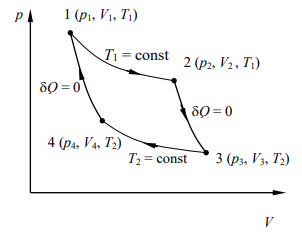
\includegraphics[width = \linewidth]{Pics/physics/lec4-8.png}
\end{figure}
Тук ще разгледаме по-подробно какво става при всеки процес.\\
(1-2) Цилиндърът с бутало, в който се намира идеален газ (работното тяло), се поставя в нагревател с температура $T_1 = const$. Газът поглъща количество топлина $Q_1$, разширява се и извършва работа. \\
(2-3) Цилиндърът се изважда от нагревателя и се изолира топлинно. Газът се
разширява адиабатно $(\delta Q = 0)$ до обем $V_3$, температурата му се понижава до $T_2$ и 
извършва работа за сметка на вътрешната си енергия.\\
(3-4) Цилиндърът се отстранява от топлинната изолация и се поставя в охладител
с температура $T_2 = const$. Газът се свива изотермно, обемът му намалява до $V_4$. \\
(4-1) Цилиндърът се изважда от охладителя и се изолира топлинно. Газът се
свива адиабатно $(\delta Q = 0)$, обемът му намалява до началната стойност $V_1$, температурата - до
$T_1$ и той се връща в изходното си състояние. \\
За коефициента на полезно действие на топлинна машина, работеща по обратимия цикъл на Карно, се получава: 
$$\eta = 1 - \frac{T_2}{T_1}$$
Основни изводи: 
\begin{enumerate}
\item к.п.д. на топлинна машина, работеща по цикъла на Карно, не зависи от вида на
работното тяло; к.п.д зависи единствено от температурата на нагревателя $T_1$ и на
охладителя $T_2$ \textbf{(първа теорема на Карно)}.
\item к.п.д за всяка реална машина е по-малък от к.п.д за обратимия цикъл на Карно \textbf{(втора теорема на Карно)}.
\end{enumerate}
По такъв начин цикълът на Карно дава горната граница на коефициента на
полезно действие на топлинните машини, работещи при дадена температура на
нагревателя и охладителя. Ако например по формулата $\eta = 1 - \frac{T_2}{T_1}$ сме изчислили $\eta = 0.4$, 
то всяка реална машина, работеща при същите температури на нагревателя и охладителя, ще има по-нисък к.п.д.

\begin{example}
Да се намери коефициента на полезно действие на топлинна машина,
работеща по обратимия цикъл на Карно с температура на нагревателя
$t_1 = 97^\circ C $ и температура на охладителя $t_2 = 27^\circ C$.\\
Решение: \\
\begin{gather*}
T_1 = t_1 + 273 = 370K \\
T_2 = t_2 + 273 = 300K \\
\eta = 1 - \frac{T_2}{T_1} = 1 - \frac{300}{370} = 0.19 = 19 \%
\end{gather*}
\end{example}

\begin{example}
Да се намери коефициента на полезно действие на топлинна машина, която 
за един цикъл получава 1000 J топлина и извършва 400 J работа.\\
Решение: \\
$$\nu = \frac{A}{Q_1} = \frac{400}{1000} = 0.4 = 40 \% $$
\end{example}

\subsection{Формулировки на втория принцип на термодинамиката}

\begin{enumerate}
\item Формулировка на Клаузиус (1850г.): \textbf{Не е възможен термодинамичен процес, 
единственият краен резултат от който да е предаване на количество топлина от
термодинамична система с по-ниска температура на термодинамична система с
по-висока температура.}
\item Формулировка на Келвин (1851г.): \textbf{Не е възможен кръгов процес,
единственият краен резултат от който е извършване на работа за сметка на
охлаждане на една термодинамична система.}
\end{enumerate}


\newpage
\section{Лекция 5: Молекулна физика}

\subsection{Основно уравнение на молекулно-кинетичната теория}
Разглеждаме газ затворен в съд. Една молекула
(условно й слагаме индекс i) с маса m се движи къмстената със скорост $v_i$. 
Импулсът и е $p_{i1} = mv_i$. Молекулата се отразява от стената еластично и се връща към газа със скорост $- v_i$
и импулсът $p_{i2} = -mv_i$. Изменението на импулса $\Delta p_i = p_{i2} - p_{i1} = -2mv_i$.
От закона за запазване на импулса стената на съда ще получи импулс $\Delta p_i = -2mv_i$.\\
След като сумираме импулса, който получава стената от всички частици, удрящи се в нея, от втория принцип на Нютон
$F = \frac{\Delta p}{\Delta t}$ можем да определим силата, действаща на стената, а от там и налягането $p = \frac{F}{S}$. \\ 
По такъв начин молекулно-кинетичната теория изяснява същността на налягането: 
то се дължи на ударите на молекулите в стените на съда. \\
Крайният резултат, който се получава е:
$$pV = \frac{1}{3} Nm \overline{v_i^2}$$
Тук N е броят на молекулите в съда, m е масата на една молекула, а $\overline{v_i}$ е
средната скорост на една молекула. (По-точно средна квадратична скорост, тъй като
осредняването е извършено след като скоростта е вдигната на квадрат) \\
Tова равенство се нарича основно уравнение на молекулно-кинетичната теория
на идеалния газ. Като имаме предвид, че средната кинетична енергия на молекулите е $\overline{E_k} = \frac{m\overline{v_i^2}}{2}$ можем да го запишем и в друга форма:
$$pV = \frac{2}{3} N \overline{E_k}$$

\subsection{Физичен смисъл на величината температура.}
Броят на молекулите в един mol е равен на числото на Авогадро $N_A$. За 1 mol:
$$pV = \frac{2}{3} N_A \overline{E_k}$$
От уравнението за състоянието на идеален газ $pV = RT$ . Като сравним двата израза получаваме $\overline{E_k} = \frac{3}{2} \frac{R}{N_A}T$. \\
Константата $k = \frac{R}{N_A} = 1.38 \cdot 10^{-23} J/K $ се нарича константа на Болцман. 
Получаваме 
$$\overline{E_k} = \frac{3}{2}kT$$
Оттук се вижда физичният смисъл на величината температура. \textbf{Температурата
е мярка за средната кинетична енергия на молекулите.} Съгласно този резултат, ако
намалим температурата на газа, ще намалее и кинетичната енергия на частиците и
тяхната скорост. При абсолютната нула $T = 0K$ според класическата теория молекулите ще спрат да се движат.

\begin{example}
Да се намери средната енергия и средната квадратична скорост на
атоми на аргон при стайна температура $(T = 300К)$. Масата на аргоновия атом е $m = 6.7 \cdot 10^{-26} kg$. \\
Решение: 
\begin{gather*}
\overline{E_k} = \frac{3}{2}kT = \frac{3}{2} \cdot  1.38 \cdot 10^{-23} \cdot 300 = 6.21 \cdot 10^{-21} J \\
\overline{E_k} = \frac{m\overline{v_i^2}}{2} \implies \overline{v_i} = \sqrt{\frac{2\overline{E_k}}{m}} = 430 m/s
\end{gather*}
\end{example}
Вътрешната енергия на идеален газ е равна на сумата от кинетичните енергии на
всички молекули: 
$$U = \sum _{i =1} ^N E_{ki} = N\overline{E_k}$$

\begin{example}
При условията на предния пример да се намери вътрешната енергия на
2 mol газ. \\
Решение:
\begin{gather*}
\overline{E_k} 6.21 \cdot 10^{-21} J \\
N_A = 6.022 \cdot 10^{23} mol^{-1} \\
U = \sum _{i =1} ^N E_{ki} = N\overline{E_k} = 2N_A \overline{E_k} = 2 \cdot 6.022 \cdot 10^{23} \cdot 6.21 \cdot 10^{-21} \approx 7500J
\end{gather*}
\end{example}
Ако бяхме разглеждали движение само в едно направление (например само по оста х) 
за средната енергия щяхме да получим $\overline{E_k} = \frac{1}{2}kT$. 
Най-общо изразът за средната енергия може да се запише във вида $\overline{E_k} = \frac{i}{2}kT$, 
като i е броят на степените на свобода. За едноатомни молекули броят на степените на свобода е равен на броя на
направленията, по които молекулата може да се движи. При многоатомни молекули се
появяват допълнителни степени на свобода, свързани с трептения на молекулата и
въртеливи движения. \\
В статистическата физика се доказва следната теорема за частиците в равновесна
термодинамична система: \textit{На всяка степен на свобода на една частица съответства
една и съща средна кинетична енергия} $\frac{1}{2}kT$ \\
От израза $p = \frac{1}{3} mn \overline{v_i ^2}$, който получихме по-горе, като заместим 
$m\overline{v_i ^2} = 2\overline{E_k}$ получаваме 
$p = \frac{2}{3}n \overline{E_k}$ и като заместим $\overline{E_k} = \frac{3}{2}kT$ се получава:
$$p = nkT$$
\begin{example}
Да се намери концентрацията на частиците на газ при атмосферно
налягане $(p =100000 Pa)$ и стайна температура $(Т = 300 К)$. \\
Решение: \\
$$p = nkT \implies n = \frac{P}{kT} = \frac{100000}{1.38 \cdot 10^{-23} \cdot 300} = 2.4 \cdot 10^{25} m^{-3}$$
\end{example}

\subsection{Функция на разпределение}
Молекулите в газовете се движат хаотично във
всички посоки с различни скорости. При удари между
молекулите скоростите на частиците се променят.
Понякога се налага да знаем каква част от молекулите
се движат с дадена скорост. Например за някои
процеси (като йонизация) са необходими частици,
имащи голяма скорост. \\
Функцията на разпределение показва каква
част от частиците се движат със скорости в някакъв
малък интервал от
v до v + dv. За случая на
термодинамично равновесие, функцията на
разпределение е била теоретично получена от
английския физик Максуел. Тя има вида: \\
$$f(v) = 4\pi(\frac{m}{2\pi kT})^{\frac{3}{2}} v^2 \exp \left({- \frac{mv^2}{2kT}}\right)$$
В този израз
m е масата намолекулите, k е константа на Болцман, 
T е температурата, $\pi = 3.14$, а exp е означение за експоненциална функция $\exp{(x)} = e^x$ \\
Като се вижда от горния израз, броят на молекулите, които са неподвижни, т.е.
имат скорост нула е нула. Също така броят на молекулите, движещи се с много голяма
скорост е много малък.\\
Функцията на разпределение зависи от температурата на газа. На фигурата е 
показана функцията на разпределение за три температури. С увеличаване на
температурата, максимумът на функцията се измества към по-високите температури.
Този резултат е в съответствие с направения по-рано извод, че температурата е мярка за
средната кинетична енергия на частиците. (по-висока температура води до по-голяма
средна енергия, а оттам до по-високи скорости на молекулите.

\subsection{Разпределение на Болцман}
До тук предполагахме, че на газа не действат външни сили. Частиците са
разпределени равномерно в целия обем. Ако действа външно поле, то може да доведе
до неравномерно разпределение на частиците. Например въздухът около Земята се
намира в полето на силата на тежестта. В резултат на това, с увеличаване на
надморската височина въздухът е по-разреден. \\
Болцман е установил, че концентрацията на частиците
n (брой частици в единица обем) зависи от потенциалната енергия на частиците
$E_p$ по следния начин:
$$n = n_0 \exp{\left( - \frac{E_p}{kT}\right)}$$
$n_0$ е концентрацията на частиците при потенциална енергия равна на нула.

\newpage
\section{Формули}

\subsection{Лекция 1}

\subsection{Лекция 2}

\subsection{Лекция 3}

\subsection{Лекция 4}

\subsection{Лекция 5}











\end{document}